\documentclass[twoside]{book}

% Packages required by doxygen
\usepackage{fixltx2e}
\usepackage{calc}
\usepackage{doxygen}
\usepackage[export]{adjustbox} % also loads graphicx
\usepackage{graphicx}
\usepackage[utf8]{inputenc}
\usepackage{makeidx}
\usepackage{multicol}
\usepackage{multirow}
\PassOptionsToPackage{warn}{textcomp}
\usepackage{textcomp}
\usepackage[nointegrals]{wasysym}
\usepackage[table]{xcolor}

% Font selection
\usepackage[T1]{fontenc}
\usepackage[scaled=.90]{helvet}
\usepackage{courier}
\usepackage{amssymb}
\usepackage{sectsty}
\renewcommand{\familydefault}{\sfdefault}
\allsectionsfont{%
  \fontseries{bc}\selectfont%
  \color{darkgray}%
}
\renewcommand{\DoxyLabelFont}{%
  \fontseries{bc}\selectfont%
  \color{darkgray}%
}
\newcommand{\+}{\discretionary{\mbox{\scriptsize$\hookleftarrow$}}{}{}}

% Page & text layout
\usepackage{geometry}
\geometry{%
  a4paper,%
  top=2.5cm,%
  bottom=2.5cm,%
  left=2.5cm,%
  right=2.5cm%
}
\tolerance=750
\hfuzz=15pt
\hbadness=750
\setlength{\emergencystretch}{15pt}
\setlength{\parindent}{0cm}
\setlength{\parskip}{3ex plus 2ex minus 2ex}
\makeatletter
\renewcommand{\paragraph}{%
  \@startsection{paragraph}{4}{0ex}{-1.0ex}{1.0ex}{%
    \normalfont\normalsize\bfseries\SS@parafont%
  }%
}
\renewcommand{\subparagraph}{%
  \@startsection{subparagraph}{5}{0ex}{-1.0ex}{1.0ex}{%
    \normalfont\normalsize\bfseries\SS@subparafont%
  }%
}
\makeatother

% Headers & footers
\usepackage{fancyhdr}
\pagestyle{fancyplain}
\fancyhead[LE]{\fancyplain{}{\bfseries\thepage}}
\fancyhead[CE]{\fancyplain{}{}}
\fancyhead[RE]{\fancyplain{}{\bfseries\leftmark}}
\fancyhead[LO]{\fancyplain{}{\bfseries\rightmark}}
\fancyhead[CO]{\fancyplain{}{}}
\fancyhead[RO]{\fancyplain{}{\bfseries\thepage}}
\fancyfoot[LE]{\fancyplain{}{}}
\fancyfoot[CE]{\fancyplain{}{}}
\fancyfoot[RE]{\fancyplain{}{\bfseries\scriptsize Generated by Doxygen }}
\fancyfoot[LO]{\fancyplain{}{\bfseries\scriptsize Generated by Doxygen }}
\fancyfoot[CO]{\fancyplain{}{}}
\fancyfoot[RO]{\fancyplain{}{}}
\renewcommand{\footrulewidth}{0.4pt}
\renewcommand{\chaptermark}[1]{%
  \markboth{#1}{}%
}
\renewcommand{\sectionmark}[1]{%
  \markright{\thesection\ #1}%
}

% Indices & bibliography
\usepackage{natbib}
\usepackage[titles]{tocloft}
\setcounter{tocdepth}{3}
\setcounter{secnumdepth}{5}
\makeindex

% Hyperlinks (required, but should be loaded last)
\usepackage{ifpdf}
\ifpdf
  \usepackage[pdftex,pagebackref=true]{hyperref}
\else
  \usepackage[ps2pdf,pagebackref=true]{hyperref}
\fi
\hypersetup{%
  colorlinks=true,%
  linkcolor=blue,%
  citecolor=blue,%
  unicode%
}

% Custom commands
\newcommand{\clearemptydoublepage}{%
  \newpage{\pagestyle{empty}\cleardoublepage}%
}

\usepackage{caption}
\captionsetup{labelsep=space,justification=centering,font={bf},singlelinecheck=off,skip=4pt,position=top}

%===== C O N T E N T S =====

\begin{document}

% Titlepage & ToC
\hypersetup{pageanchor=false,
             bookmarksnumbered=true,
             pdfencoding=unicode
            }
\pagenumbering{alph}
\begin{titlepage}
\vspace*{7cm}
\begin{center}%
{\Large Doxygen Testing }\\
\vspace*{1cm}
{\large Generated by Doxygen 1.8.13}\\
\end{center}
\end{titlepage}
\clearemptydoublepage
\pagenumbering{roman}
\tableofcontents
\clearemptydoublepage
\pagenumbering{arabic}
\hypersetup{pageanchor=true}

%--- Begin generated contents ---
\chapter{R\+E\+A\+D\+ME}
\label{md_README}
\Hypertarget{md_README}
\input{md_README}
\chapter{Hierarchical Index}
\section{Class Hierarchy}
This inheritance list is sorted roughly, but not completely, alphabetically\+:\begin{DoxyCompactList}
\item \contentsline{section}{Employee}{\pageref{classEmployee}}{}
\begin{DoxyCompactList}
\item \contentsline{section}{Officer}{\pageref{classOfficer}}{}
\item \contentsline{section}{Supervisor}{\pageref{classSupervisor}}{}
\end{DoxyCompactList}
\end{DoxyCompactList}

\chapter{Class Index}
\section{Class List}
Here are the classes, structs, unions and interfaces with brief descriptions\+:\begin{DoxyCompactList}
\item\contentsline{section}{\hyperlink{classEmployee}{Employee} \\*\hyperlink{classEmployee}{Employee} class }{\pageref{classEmployee}}{}
\item\contentsline{section}{\hyperlink{classOfficer}{Officer} \\*\hyperlink{classOfficer}{Officer} class expanding on \hyperlink{classEmployee}{Employee} subclass }{\pageref{classOfficer}}{}
\item\contentsline{section}{\hyperlink{classSupervisor}{Supervisor} \\*\hyperlink{classSupervisor}{Supervisor} class expanding on \hyperlink{classEmployee}{Employee} subclass }{\pageref{classSupervisor}}{}
\end{DoxyCompactList}

\chapter{File Index}
\section{File List}
Here is a list of all documented files with brief descriptions\+:\begin{DoxyCompactList}
\item\contentsline{section}{\hyperlink{Employee_8cpp}{Employee.\+cpp} \\*\hyperlink{classEmployee}{Employee} implementation }{\pageref{Employee_8cpp}}{}
\item\contentsline{section}{\hyperlink{Employee_8h}{Employee.\+h} \\*\hyperlink{classEmployee}{Employee} class header file }{\pageref{Employee_8h}}{}
\item\contentsline{section}{\hyperlink{main_8cpp}{main.\+cpp} \\*Driver file for \hyperlink{classEmployee}{Employee} project }{\pageref{main_8cpp}}{}
\item\contentsline{section}{\hyperlink{Officer_8cpp}{Officer.\+cpp} \\*\hyperlink{classOfficer}{Officer} implementation file }{\pageref{Officer_8cpp}}{}
\item\contentsline{section}{\hyperlink{Officer_8h}{Officer.\+h} \\*\hyperlink{classOfficer}{Officer} header file }{\pageref{Officer_8h}}{}
\item\contentsline{section}{\hyperlink{Supervisor_8cpp}{Supervisor.\+cpp} \\*\hyperlink{classSupervisor}{Supervisor} implementation file }{\pageref{Supervisor_8cpp}}{}
\item\contentsline{section}{\hyperlink{Supervisor_8h}{Supervisor.\+h} \\*\hyperlink{classSupervisor}{Supervisor} header file }{\pageref{Supervisor_8h}}{}
\end{DoxyCompactList}

\chapter{Class Documentation}
\hypertarget{classEmployee}{}\section{Employee Class Reference}
\label{classEmployee}\index{Employee@{Employee}}


employee class  




{\ttfamily \#include \char`\"{}Doxygen/\+Employee.\+h\char`\"{}}



Inheritance diagram for Employee\+:\nopagebreak
\begin{figure}[H]
\begin{center}
\leavevmode
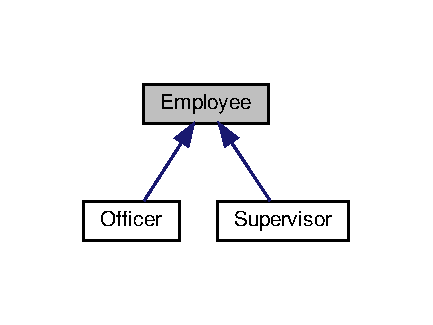
\includegraphics[width=208pt]{classEmployee__inherit__graph}
\end{center}
\end{figure}
\subsection*{Public Member Functions}
\begin{DoxyCompactItemize}
\item 
virtual void \hyperlink{classEmployee_a79556ad700627dba88049f487a34a762}{print} ()
\item 
virtual double \hyperlink{classEmployee_a01c2c44e15434237db28832f6972e960}{calculate\+Pay} ()
\item 
void \hyperlink{classEmployee_a67c345031cf63f515fb09dc675dee5f3}{anniversary} ()
\item 
\hyperlink{classEmployee_a003c7bd08c40924e381eb0750cbb906f}{Employee} ()
\item 
\hyperlink{classEmployee_ad0c935ef9a290a82dcf7865172c90148}{Employee} (int ID, int years, double hourly\+Rate, float hours\+Worked)
\end{DoxyCompactItemize}
\subsection*{Protected Attributes}
\begin{DoxyCompactItemize}
\item 
\mbox{\Hypertarget{classEmployee_ac31134abb9b4004fc015e51ef579b069}\label{classEmployee_ac31134abb9b4004fc015e51ef579b069}} 
double {\bfseries hourly\+Rate}
\item 
\mbox{\Hypertarget{classEmployee_afde35c73d02eb1cfe89e23a80998b42e}\label{classEmployee_afde35c73d02eb1cfe89e23a80998b42e}} 
float {\bfseries hours\+Worked}
\end{DoxyCompactItemize}
\subsection*{Private Attributes}
\begin{DoxyCompactItemize}
\item 
\mbox{\Hypertarget{classEmployee_a832bbae4ee8a704b917f82c4d497bbac}\label{classEmployee_a832bbae4ee8a704b917f82c4d497bbac}} 
int {\bfseries ID}
\item 
\mbox{\Hypertarget{classEmployee_a3e4862d9dfc73becb459a562fa2e25f5}\label{classEmployee_a3e4862d9dfc73becb459a562fa2e25f5}} 
int {\bfseries years}
\end{DoxyCompactItemize}


\subsection{Detailed Description}
employee class 

base employee class has an ID and years worked, as well as the ability to calculate pay 

\subsection{Constructor \& Destructor Documentation}
\mbox{\Hypertarget{classEmployee_a003c7bd08c40924e381eb0750cbb906f}\label{classEmployee_a003c7bd08c40924e381eb0750cbb906f}} 
\index{Employee@{Employee}!Employee@{Employee}}
\index{Employee@{Employee}!Employee@{Employee}}
\subsubsection{\texorpdfstring{Employee()}{Employee()}\hspace{0.1cm}{\footnotesize\ttfamily [1/2]}}
{\footnotesize\ttfamily Employee\+::\+Employee (\begin{DoxyParamCaption}{ }\end{DoxyParamCaption})}

default constructor

\begin{DoxyPostcond}{Postcondition}
all data members initialized to -\/1 
\end{DoxyPostcond}
\mbox{\Hypertarget{classEmployee_ad0c935ef9a290a82dcf7865172c90148}\label{classEmployee_ad0c935ef9a290a82dcf7865172c90148}} 
\index{Employee@{Employee}!Employee@{Employee}}
\index{Employee@{Employee}!Employee@{Employee}}
\subsubsection{\texorpdfstring{Employee()}{Employee()}\hspace{0.1cm}{\footnotesize\ttfamily [2/2]}}
{\footnotesize\ttfamily Employee\+::\+Employee (\begin{DoxyParamCaption}\item[{int}]{ID,  }\item[{int}]{years,  }\item[{double}]{hourly\+Rate,  }\item[{float}]{hours\+Worked }\end{DoxyParamCaption})}

parameterized constructor


\begin{DoxyParams}{Parameters}
{\em int} & ID employee ID number \\
\hline
{\em int} & years years worked at the company thus far \\
\hline
{\em double} & hourly\+Rate hourly rate employee is paid \\
\hline
{\em float} & hours\+Worked hours worked during a week \\
\hline
\end{DoxyParams}


\subsection{Member Function Documentation}
\mbox{\Hypertarget{classEmployee_a67c345031cf63f515fb09dc675dee5f3}\label{classEmployee_a67c345031cf63f515fb09dc675dee5f3}} 
\index{Employee@{Employee}!anniversary@{anniversary}}
\index{anniversary@{anniversary}!Employee@{Employee}}
\subsubsection{\texorpdfstring{anniversary()}{anniversary()}}
{\footnotesize\ttfamily void Employee\+::anniversary (\begin{DoxyParamCaption}{ }\end{DoxyParamCaption})}

increases employee\textquotesingle{}s years worked at company, and increases their pay tremendously, as well as printing a congratulatory message to console

\begin{DoxyReturn}{Returns}
void 
\end{DoxyReturn}
\begin{DoxyPostcond}{Postcondition}
years worked and pay increased, and congratulations printed to console 
\end{DoxyPostcond}


Referenced by run\+Employee\+Tests().

\mbox{\Hypertarget{classEmployee_a01c2c44e15434237db28832f6972e960}\label{classEmployee_a01c2c44e15434237db28832f6972e960}} 
\index{Employee@{Employee}!calculate\+Pay@{calculate\+Pay}}
\index{calculate\+Pay@{calculate\+Pay}!Employee@{Employee}}
\subsubsection{\texorpdfstring{calculate\+Pay()}{calculatePay()}}
{\footnotesize\ttfamily double Employee\+::calculate\+Pay (\begin{DoxyParamCaption}{ }\end{DoxyParamCaption})\hspace{0.3cm}{\ttfamily [virtual]}}

calculates the pay the employee is owed for hours worked

\begin{DoxyReturn}{Returns}
double amount in dollars calculated for employee\textquotesingle{}s work 
\end{DoxyReturn}


Reimplemented in \hyperlink{classOfficer_a1fa1aad39b9e95be7a088990ebf17059}{Officer}, and \hyperlink{classSupervisor_aa37daa89523c08b84ae8141299e036f8}{Supervisor}.



Referenced by Supervisor\+::calculate\+Pay(), and run\+Employee\+Tests().

\mbox{\Hypertarget{classEmployee_a79556ad700627dba88049f487a34a762}\label{classEmployee_a79556ad700627dba88049f487a34a762}} 
\index{Employee@{Employee}!print@{print}}
\index{print@{print}!Employee@{Employee}}
\subsubsection{\texorpdfstring{print()}{print()}}
{\footnotesize\ttfamily void Employee\+::print (\begin{DoxyParamCaption}{ }\end{DoxyParamCaption})\hspace{0.3cm}{\ttfamily [virtual]}}

prints out employee information to console

\begin{DoxyReturn}{Returns}
void 
\end{DoxyReturn}
\begin{DoxyPostcond}{Postcondition}
employee information printed to console 
\end{DoxyPostcond}


Reimplemented in \hyperlink{classOfficer_aeadece05a1a0b7fb29bd412830d2e07a}{Officer}, and \hyperlink{classSupervisor_a92483dc9a54904d79b46c6ec4efb3f54}{Supervisor}.



Referenced by Supervisor\+::print(), Officer\+::print(), and run\+Employee\+Tests().



The documentation for this class was generated from the following files\+:\begin{DoxyCompactItemize}
\item 
\hyperlink{Employee_8h}{Employee.\+h}\item 
\hyperlink{Employee_8cpp}{Employee.\+cpp}\end{DoxyCompactItemize}

\hypertarget{classOfficer}{}\section{Officer Class Reference}
\label{classOfficer}\index{Officer@{Officer}}


\hyperlink{classOfficer}{Officer} class expanding on \hyperlink{classEmployee}{Employee} subclass.  




{\ttfamily \#include \char`\"{}Doxygen/\+Officer.\+h\char`\"{}}



Inheritance diagram for Officer\+:\nopagebreak
\begin{figure}[H]
\begin{center}
\leavevmode
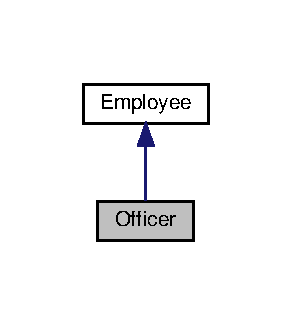
\includegraphics[width=140pt]{classOfficer__inherit__graph}
\end{center}
\end{figure}


Collaboration diagram for Officer\+:\nopagebreak
\begin{figure}[H]
\begin{center}
\leavevmode
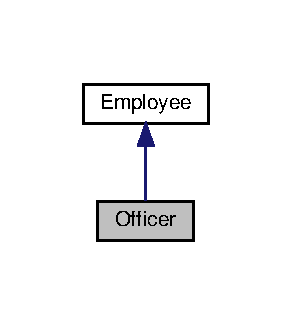
\includegraphics[width=140pt]{classOfficer__coll__graph}
\end{center}
\end{figure}
\subsection*{Public Member Functions}
\begin{DoxyCompactItemize}
\item 
void \hyperlink{classOfficer_aeadece05a1a0b7fb29bd412830d2e07a}{print} ()
\item 
double \hyperlink{classOfficer_a1fa1aad39b9e95be7a088990ebf17059}{calculate\+Pay} ()
\item 
\hyperlink{classOfficer_a80ac1e36a3f36c3a7e12b5dc9320ad89}{Officer} ()
\item 
\hyperlink{classOfficer_ac75c45d6e8628606278cb4ce6596f67f}{Officer} (int ID, int years, double hourly\+Rate, float hours\+Worked, double evilness)
\end{DoxyCompactItemize}
\subsection*{Private Attributes}
\begin{DoxyCompactItemize}
\item 
\mbox{\Hypertarget{classOfficer_a63465c5f16e8148e5bc0a3bb4ecd1781}\label{classOfficer_a63465c5f16e8148e5bc0a3bb4ecd1781}} 
double {\bfseries evilness}
\end{DoxyCompactItemize}
\subsection*{Additional Inherited Members}


\subsection{Detailed Description}
\hyperlink{classOfficer}{Officer} class expanding on \hyperlink{classEmployee}{Employee} subclass. 

the officer is a type of employee with an added evilness and a pay befitting their hard work 

\subsection{Constructor \& Destructor Documentation}
\mbox{\Hypertarget{classOfficer_a80ac1e36a3f36c3a7e12b5dc9320ad89}\label{classOfficer_a80ac1e36a3f36c3a7e12b5dc9320ad89}} 
\index{Officer@{Officer}!Officer@{Officer}}
\index{Officer@{Officer}!Officer@{Officer}}
\subsubsection{\texorpdfstring{Officer()}{Officer()}\hspace{0.1cm}{\footnotesize\ttfamily [1/2]}}
{\footnotesize\ttfamily Officer\+::\+Officer (\begin{DoxyParamCaption}{ }\end{DoxyParamCaption})}

default constructor, evilness is set to 500 \mbox{\Hypertarget{classOfficer_ac75c45d6e8628606278cb4ce6596f67f}\label{classOfficer_ac75c45d6e8628606278cb4ce6596f67f}} 
\index{Officer@{Officer}!Officer@{Officer}}
\index{Officer@{Officer}!Officer@{Officer}}
\subsubsection{\texorpdfstring{Officer()}{Officer()}\hspace{0.1cm}{\footnotesize\ttfamily [2/2]}}
{\footnotesize\ttfamily Officer\+::\+Officer (\begin{DoxyParamCaption}\item[{int}]{ID,  }\item[{int}]{years,  }\item[{double}]{hourly\+Rate,  }\item[{float}]{hours\+Worked,  }\item[{double}]{evilness }\end{DoxyParamCaption})}

parameterized constructor, data members set to entered values


\begin{DoxyParams}{Parameters}
{\em int} & ID ID of officer \\
\hline
{\em int} & years years worked at the company \\
\hline
{\em double} & hourly\+Rate pay per hour worked \\
\hline
{\em float} & hours\+Worked hours worked in a pay period \\
\hline
{\em double} & evilness blackness of the heart, more evilness means greater pay \\
\hline
\end{DoxyParams}


\subsection{Member Function Documentation}
\mbox{\Hypertarget{classOfficer_a1fa1aad39b9e95be7a088990ebf17059}\label{classOfficer_a1fa1aad39b9e95be7a088990ebf17059}} 
\index{Officer@{Officer}!calculate\+Pay@{calculate\+Pay}}
\index{calculate\+Pay@{calculate\+Pay}!Officer@{Officer}}
\subsubsection{\texorpdfstring{calculate\+Pay()}{calculatePay()}}
{\footnotesize\ttfamily double Officer\+::calculate\+Pay (\begin{DoxyParamCaption}{ }\end{DoxyParamCaption})\hspace{0.3cm}{\ttfamily [virtual]}}

calculates amount of pay officer is owed

\begin{DoxyReturn}{Returns}
double pay officer is owed in dollars 
\end{DoxyReturn}


Reimplemented from \hyperlink{classEmployee_a01c2c44e15434237db28832f6972e960}{Employee}.

\mbox{\Hypertarget{classOfficer_aeadece05a1a0b7fb29bd412830d2e07a}\label{classOfficer_aeadece05a1a0b7fb29bd412830d2e07a}} 
\index{Officer@{Officer}!print@{print}}
\index{print@{print}!Officer@{Officer}}
\subsubsection{\texorpdfstring{print()}{print()}}
{\footnotesize\ttfamily void Officer\+::print (\begin{DoxyParamCaption}{ }\end{DoxyParamCaption})\hspace{0.3cm}{\ttfamily [virtual]}}

prints out officer information to console

\begin{DoxyReturn}{Returns}
void 
\end{DoxyReturn}
\begin{DoxyPostcond}{Postcondition}
officer information printed to console 
\end{DoxyPostcond}


Reimplemented from \hyperlink{classEmployee_a79556ad700627dba88049f487a34a762}{Employee}.



The documentation for this class was generated from the following files\+:\begin{DoxyCompactItemize}
\item 
\hyperlink{Officer_8h}{Officer.\+h}\item 
\hyperlink{Officer_8cpp}{Officer.\+cpp}\end{DoxyCompactItemize}

\hypertarget{classSupervisor}{}\section{Supervisor Class Reference}
\label{classSupervisor}\index{Supervisor@{Supervisor}}


\hyperlink{classSupervisor}{Supervisor} class expanding on \hyperlink{classEmployee}{Employee} subclass.  




{\ttfamily \#include \char`\"{}Doxygen/\+Supervisor.\+h\char`\"{}}



Inheritance diagram for Supervisor\+:\nopagebreak
\begin{figure}[H]
\begin{center}
\leavevmode
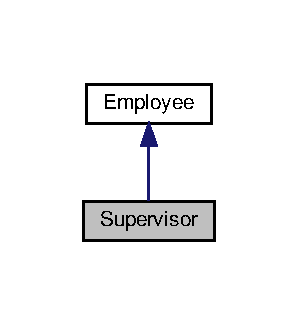
\includegraphics[width=143pt]{classSupervisor__inherit__graph}
\end{center}
\end{figure}


Collaboration diagram for Supervisor\+:\nopagebreak
\begin{figure}[H]
\begin{center}
\leavevmode
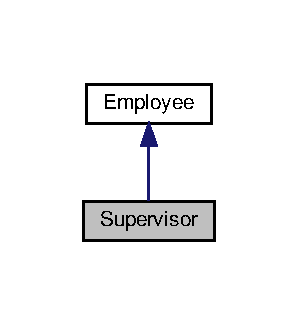
\includegraphics[width=143pt]{classSupervisor__coll__graph}
\end{center}
\end{figure}
\subsection*{Public Member Functions}
\begin{DoxyCompactItemize}
\item 
void \hyperlink{classSupervisor_a92483dc9a54904d79b46c6ec4efb3f54}{print} ()
\item 
double \hyperlink{classSupervisor_aa37daa89523c08b84ae8141299e036f8}{calculate\+Pay} ()
\item 
\hyperlink{classSupervisor_a9d7eafc36b5429092ba0f758bc7841c4}{Supervisor} ()
\item 
\hyperlink{classSupervisor_a02d9245744652deb20e9408001d6ed3b}{Supervisor} (int ID, int years, double hourly\+Rate, float hours\+Worked, int num\+Supervised)
\end{DoxyCompactItemize}
\subsection*{Private Attributes}
\begin{DoxyCompactItemize}
\item 
\mbox{\Hypertarget{classSupervisor_af8b7097d8147c93a68d1f63c5b898797}\label{classSupervisor_af8b7097d8147c93a68d1f63c5b898797}} 
int {\bfseries num\+Supervised}
\end{DoxyCompactItemize}
\subsection*{Additional Inherited Members}


\subsection{Detailed Description}
\hyperlink{classSupervisor}{Supervisor} class expanding on \hyperlink{classEmployee}{Employee} subclass. 

the supervisor is an employee with the added responsibilities of taking care of other employees and increased pay 

\subsection{Constructor \& Destructor Documentation}
\mbox{\Hypertarget{classSupervisor_a9d7eafc36b5429092ba0f758bc7841c4}\label{classSupervisor_a9d7eafc36b5429092ba0f758bc7841c4}} 
\index{Supervisor@{Supervisor}!Supervisor@{Supervisor}}
\index{Supervisor@{Supervisor}!Supervisor@{Supervisor}}
\subsubsection{\texorpdfstring{Supervisor()}{Supervisor()}\hspace{0.1cm}{\footnotesize\ttfamily [1/2]}}
{\footnotesize\ttfamily Supervisor\+::\+Supervisor (\begin{DoxyParamCaption}{ }\end{DoxyParamCaption})}

default constructor, number of supervised employees defaults to -\/1 \mbox{\Hypertarget{classSupervisor_a02d9245744652deb20e9408001d6ed3b}\label{classSupervisor_a02d9245744652deb20e9408001d6ed3b}} 
\index{Supervisor@{Supervisor}!Supervisor@{Supervisor}}
\index{Supervisor@{Supervisor}!Supervisor@{Supervisor}}
\subsubsection{\texorpdfstring{Supervisor()}{Supervisor()}\hspace{0.1cm}{\footnotesize\ttfamily [2/2]}}
{\footnotesize\ttfamily Supervisor\+::\+Supervisor (\begin{DoxyParamCaption}\item[{int}]{ID,  }\item[{int}]{years,  }\item[{double}]{hourly\+Rate,  }\item[{float}]{hours\+Worked,  }\item[{int}]{num\+Supervised }\end{DoxyParamCaption})}

parameterized constructor, data members set to entered values


\begin{DoxyParams}{Parameters}
{\em int} & ID ID of supervisor \\
\hline
{\em int} & years years worked at the company \\
\hline
{\em double} & hourly\+Rate pay per hour worked \\
\hline
{\em float} & hours\+Worked hours worked in a pay period \\
\hline
{\em int} & num\+Supervised number of employees supervisor is responsible for, slightly increases pay \\
\hline
\end{DoxyParams}


\subsection{Member Function Documentation}
\mbox{\Hypertarget{classSupervisor_aa37daa89523c08b84ae8141299e036f8}\label{classSupervisor_aa37daa89523c08b84ae8141299e036f8}} 
\index{Supervisor@{Supervisor}!calculate\+Pay@{calculate\+Pay}}
\index{calculate\+Pay@{calculate\+Pay}!Supervisor@{Supervisor}}
\subsubsection{\texorpdfstring{calculate\+Pay()}{calculatePay()}}
{\footnotesize\ttfamily double Supervisor\+::calculate\+Pay (\begin{DoxyParamCaption}{ }\end{DoxyParamCaption})\hspace{0.3cm}{\ttfamily [virtual]}}

calculates the amount of pay the supervisor is owed

\begin{DoxyReturn}{Returns}
double pay supervisor is owed in dollars 
\end{DoxyReturn}


Reimplemented from \hyperlink{classEmployee_a01c2c44e15434237db28832f6972e960}{Employee}.

\mbox{\Hypertarget{classSupervisor_a92483dc9a54904d79b46c6ec4efb3f54}\label{classSupervisor_a92483dc9a54904d79b46c6ec4efb3f54}} 
\index{Supervisor@{Supervisor}!print@{print}}
\index{print@{print}!Supervisor@{Supervisor}}
\subsubsection{\texorpdfstring{print()}{print()}}
{\footnotesize\ttfamily void Supervisor\+::print (\begin{DoxyParamCaption}{ }\end{DoxyParamCaption})\hspace{0.3cm}{\ttfamily [virtual]}}

prints out supervisor information to console, including number of employees supervised

\begin{DoxyReturn}{Returns}
void 
\end{DoxyReturn}


Reimplemented from \hyperlink{classEmployee_a79556ad700627dba88049f487a34a762}{Employee}.



The documentation for this class was generated from the following files\+:\begin{DoxyCompactItemize}
\item 
\hyperlink{Supervisor_8h}{Supervisor.\+h}\item 
\hyperlink{Supervisor_8cpp}{Supervisor.\+cpp}\end{DoxyCompactItemize}

\chapter{File Documentation}
\hypertarget{Employee_8cpp}{}\section{Employee.\+cpp File Reference}
\label{Employee_8cpp}\index{Employee.\+cpp@{Employee.\+cpp}}


employee implementation  


{\ttfamily \#include \char`\"{}Employee.\+h\char`\"{}}\newline
{\ttfamily \#include $<$iostream$>$}\newline
Include dependency graph for Employee.\+cpp\+:\nopagebreak
\begin{figure}[H]
\begin{center}
\leavevmode
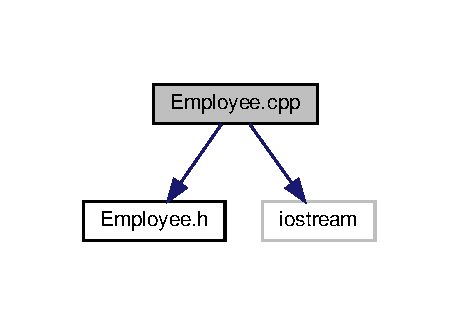
\includegraphics[width=220pt]{Employee_8cpp__incl}
\end{center}
\end{figure}


\subsection{Detailed Description}
employee implementation 

\begin{DoxyAuthor}{Author}
Zachary Rose 
\end{DoxyAuthor}
\begin{DoxyDate}{Date}
2022-\/11-\/14 implementation of the base employee class 
\end{DoxyDate}

\hypertarget{Employee_8h}{}\section{Employee.\+h File Reference}
\label{Employee_8h}\index{Employee.\+h@{Employee.\+h}}


employee class header file  


This graph shows which files directly or indirectly include this file\+:
\nopagebreak
\begin{figure}[H]
\begin{center}
\leavevmode
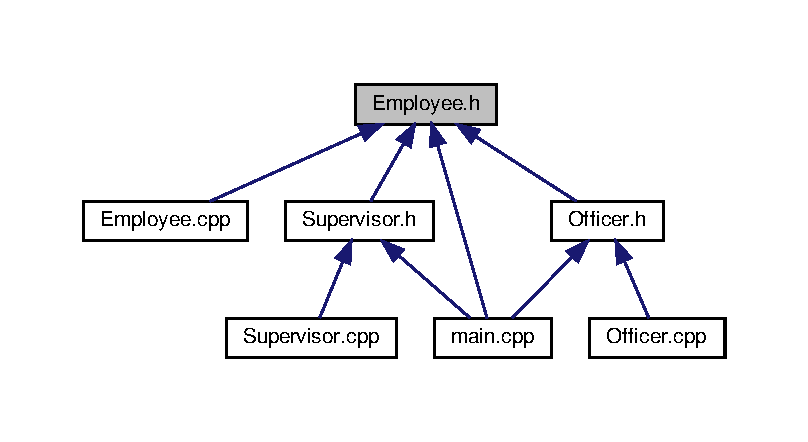
\includegraphics[width=350pt]{Employee_8h__dep__incl}
\end{center}
\end{figure}
\subsection*{Classes}
\begin{DoxyCompactItemize}
\item 
class \hyperlink{classEmployee}{Employee}
\begin{DoxyCompactList}\small\item\em employee class \end{DoxyCompactList}\end{DoxyCompactItemize}


\subsection{Detailed Description}
employee class header file 

\begin{DoxyAuthor}{Author}
Zachary Rose 
\end{DoxyAuthor}
\begin{DoxyDate}{Date}
2022-\/11-\/14 base employee class has an ID and years worked, as well as ability to calculate pay 
\end{DoxyDate}

\hypertarget{main_8cpp}{}\section{main.\+cpp File Reference}
\label{main_8cpp}\index{main.\+cpp@{main.\+cpp}}


driver file for \hyperlink{classEmployee}{Employee} project  


{\ttfamily \#include $<$iostream$>$}\newline
{\ttfamily \#include \char`\"{}Employee.\+h\char`\"{}}\newline
{\ttfamily \#include \char`\"{}Supervisor.\+h\char`\"{}}\newline
{\ttfamily \#include \char`\"{}Officer.\+h\char`\"{}}\newline
Include dependency graph for main.\+cpp\+:
\nopagebreak
\begin{figure}[H]
\begin{center}
\leavevmode
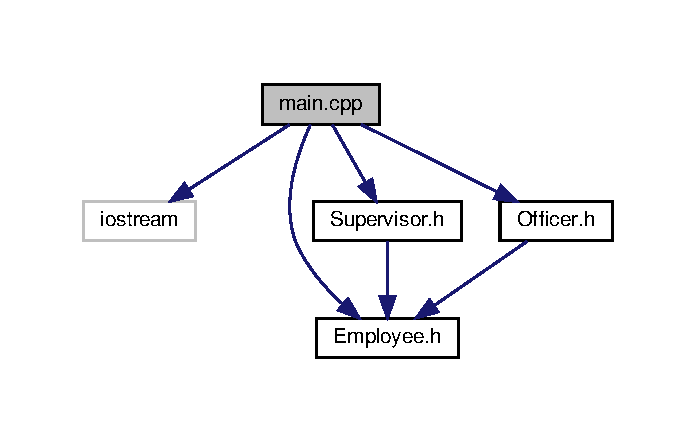
\includegraphics[width=334pt]{main_8cpp__incl}
\end{center}
\end{figure}
\subsection*{Functions}
\begin{DoxyCompactItemize}
\item 
void \hyperlink{main_8cpp_a9ccea1912d6e2275d5612e294919d113}{run\+Employee\+Tests} (\hyperlink{classEmployee}{Employee} \&e)
\item 
\mbox{\Hypertarget{main_8cpp_ae66f6b31b5ad750f1fe042a706a4e3d4}\label{main_8cpp_ae66f6b31b5ad750f1fe042a706a4e3d4}} 
int {\bfseries main} ()
\end{DoxyCompactItemize}


\subsection{Detailed Description}
driver file for \hyperlink{classEmployee}{Employee} project 

\begin{DoxyAuthor}{Author}
Zachary Rose 
\end{DoxyAuthor}
\begin{DoxyDate}{Date}
2022-\/11-\/15 driver for testing the \hyperlink{classEmployee}{Employee} project\textquotesingle{}s inheritence based classes 
\end{DoxyDate}


\subsection{Function Documentation}
\mbox{\Hypertarget{main_8cpp_a9ccea1912d6e2275d5612e294919d113}\label{main_8cpp_a9ccea1912d6e2275d5612e294919d113}} 
\index{main.\+cpp@{main.\+cpp}!run\+Employee\+Tests@{run\+Employee\+Tests}}
\index{run\+Employee\+Tests@{run\+Employee\+Tests}!main.\+cpp@{main.\+cpp}}
\subsubsection{\texorpdfstring{run\+Employee\+Tests()}{runEmployeeTests()}}
{\footnotesize\ttfamily void run\+Employee\+Tests (\begin{DoxyParamCaption}\item[{\hyperlink{classEmployee}{Employee} \&}]{e }\end{DoxyParamCaption})}

Tests the shared functions of the \hyperlink{classEmployee}{Employee} based superclasses such as printing, pay calculation, and the anniversary function


\begin{DoxyParams}{Parameters}
{\em \hyperlink{classEmployee}{Employee}} & \& e An \hyperlink{classEmployee}{Employee}, \hyperlink{classOfficer}{Officer}, or \hyperlink{classSupervisor}{Supervisor} object to test the functions of \\
\hline
\end{DoxyParams}
\begin{DoxyReturn}{Returns}
void 
\end{DoxyReturn}
\begin{DoxyPostcond}{Postcondition}
Console has printed output of the employee, and the employee has had aniversary() called, increasing years worked by one 
\end{DoxyPostcond}

\hypertarget{Officer_8cpp}{}\section{Officer.\+cpp File Reference}
\label{Officer_8cpp}\index{Officer.\+cpp@{Officer.\+cpp}}


\hyperlink{classOfficer}{Officer} implementation file.  


{\ttfamily \#include \char`\"{}Officer.\+h\char`\"{}}\newline
{\ttfamily \#include $<$iostream$>$}\newline
Include dependency graph for Officer.\+cpp\+:\nopagebreak
\begin{figure}[H]
\begin{center}
\leavevmode
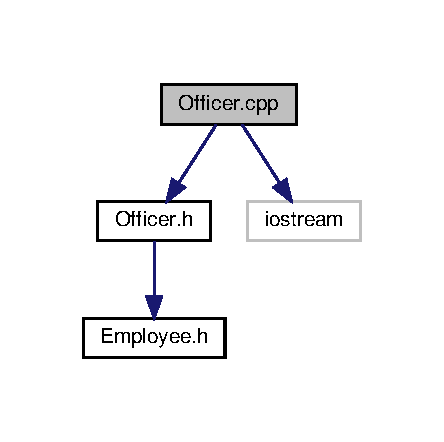
\includegraphics[width=213pt]{Officer_8cpp__incl}
\end{center}
\end{figure}


\subsection{Detailed Description}
\hyperlink{classOfficer}{Officer} implementation file. 

\begin{DoxyAuthor}{Author}
Zachary Rose 
\end{DoxyAuthor}
\begin{DoxyDate}{Date}
2022-\/11-\/15 \hyperlink{classOfficer}{Officer} implementation, superclass to \hyperlink{classEmployee}{Employee} with added evilness 
\end{DoxyDate}

\hypertarget{Officer_8h}{}\section{Officer.\+h File Reference}
\label{Officer_8h}\index{Officer.\+h@{Officer.\+h}}


officer header file  


{\ttfamily \#include \char`\"{}Employee.\+h\char`\"{}}\newline
Include dependency graph for Officer.\+h\+:\nopagebreak
\begin{figure}[H]
\begin{center}
\leavevmode
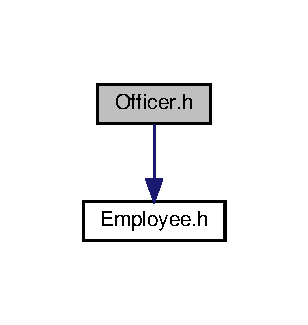
\includegraphics[width=148pt]{Officer_8h__incl}
\end{center}
\end{figure}
This graph shows which files directly or indirectly include this file\+:
\nopagebreak
\begin{figure}[H]
\begin{center}
\leavevmode
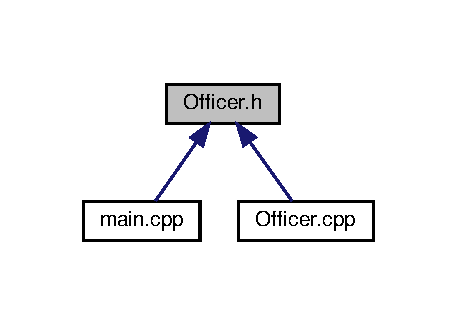
\includegraphics[width=220pt]{Officer_8h__dep__incl}
\end{center}
\end{figure}
\subsection*{Classes}
\begin{DoxyCompactItemize}
\item 
class \hyperlink{classOfficer}{Officer}
\begin{DoxyCompactList}\small\item\em \hyperlink{classOfficer}{Officer} class expanding on \hyperlink{classEmployee}{Employee} subclass. \end{DoxyCompactList}\end{DoxyCompactItemize}


\subsection{Detailed Description}
officer header file 

\begin{DoxyAuthor}{Author}
Zachary Rose 
\end{DoxyAuthor}
\begin{DoxyDate}{Date}
2022-\/11-\/15 the officer is a type of employee with an added evilness and a pay befitting their hard work 
\end{DoxyDate}

\hypertarget{Supervisor_8cpp}{}\section{Supervisor.\+cpp File Reference}
\label{Supervisor_8cpp}\index{Supervisor.\+cpp@{Supervisor.\+cpp}}


\hyperlink{classSupervisor}{Supervisor} implementation file.  


{\ttfamily \#include \char`\"{}Supervisor.\+h\char`\"{}}\newline
{\ttfamily \#include $<$iostream$>$}\newline
Include dependency graph for Supervisor.\+cpp\+:\nopagebreak
\begin{figure}[H]
\begin{center}
\leavevmode
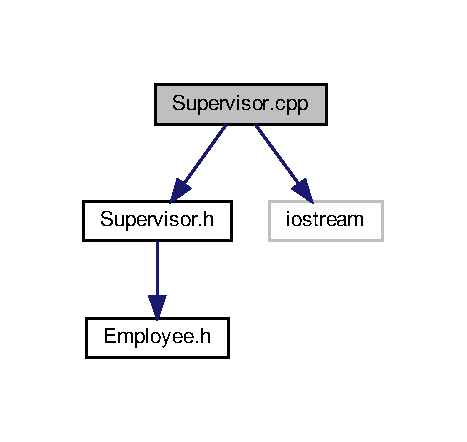
\includegraphics[width=224pt]{Supervisor_8cpp__incl}
\end{center}
\end{figure}


\subsection{Detailed Description}
\hyperlink{classSupervisor}{Supervisor} implementation file. 

\begin{DoxyAuthor}{Author}
Zachary Rose 
\end{DoxyAuthor}
\begin{DoxyDate}{Date}
2022-\/11-\/15 \hyperlink{classSupervisor}{Supervisor} implementation, superclass to \hyperlink{classEmployee}{Employee} with added supervising responsibilities 
\end{DoxyDate}

\hypertarget{Supervisor_8h}{}\section{Supervisor.\+h File Reference}
\label{Supervisor_8h}\index{Supervisor.\+h@{Supervisor.\+h}}


\hyperlink{classSupervisor}{Supervisor} header file.  


{\ttfamily \#include \char`\"{}Employee.\+h\char`\"{}}\newline
Include dependency graph for Supervisor.\+h\+:\nopagebreak
\begin{figure}[H]
\begin{center}
\leavevmode
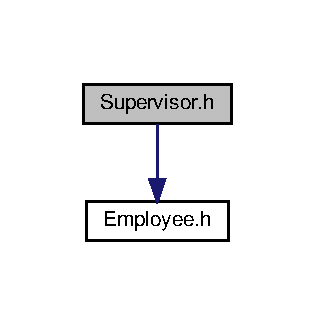
\includegraphics[width=151pt]{Supervisor_8h__incl}
\end{center}
\end{figure}
This graph shows which files directly or indirectly include this file\+:
\nopagebreak
\begin{figure}[H]
\begin{center}
\leavevmode
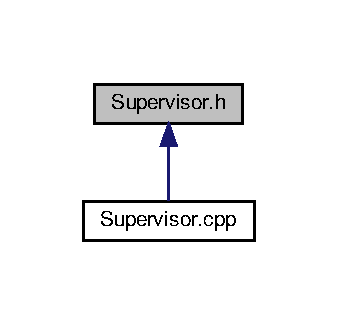
\includegraphics[width=236pt]{Supervisor_8h__dep__incl}
\end{center}
\end{figure}
\subsection*{Classes}
\begin{DoxyCompactItemize}
\item 
class \hyperlink{classSupervisor}{Supervisor}
\begin{DoxyCompactList}\small\item\em \hyperlink{classSupervisor}{Supervisor} class expanding on \hyperlink{classEmployee}{Employee} subclass. \end{DoxyCompactList}\end{DoxyCompactItemize}


\subsection{Detailed Description}
\hyperlink{classSupervisor}{Supervisor} header file. 

\begin{DoxyAuthor}{Author}
Zachary Rose 
\end{DoxyAuthor}
\begin{DoxyDate}{Date}
2022-\/11-\/15 the supervisor is an employee with the added responsibilities of taking care of other employees and increased pay 
\end{DoxyDate}

%--- End generated contents ---

% Index
\backmatter
\newpage
\phantomsection
\clearemptydoublepage
\addcontentsline{toc}{chapter}{Index}
\printindex

\end{document}
